%===============================================================================
% CareSync - AI-Powered Hospital Triage System
% Hackathon Presentation by Team KludgeKings
% Modern Minimalist Design
%===============================================================================
\documentclass[aspectratio=169,9pt]{beamer}

%-------------------------------------------------------------------------------
% PACKAGES
%-------------------------------------------------------------------------------
\usepackage[utf8]{inputenc}
\usepackage[T1]{fontenc}
\usepackage{sourcesanspro}                     % Clean sans-serif (Poppins-like)
\usepackage{graphicx}
\usepackage{booktabs}
\usepackage{array}
\usepackage{tabularx}
\usepackage{colortbl}
\usepackage{multirow}
\usepackage{tikz}
\usepackage{fontawesome5}
\usepackage{xcolor}
\usepackage{tcolorbox}
\usepackage{hyperref}

\usetikzlibrary{shapes,arrows,positioning,calc,shadows}

%-------------------------------------------------------------------------------
% CARESYNC COLOR PALETTE (Extracted from App CSS)
%-------------------------------------------------------------------------------
\usetheme{default}
\usecolortheme{default}

% Primary - Teal (CareSync brand)
\definecolor{primary}{RGB}{78,189,184}         % #4EBDB8 - Main teal
\definecolor{primarydark}{RGB}{62,168,163}     % #3EA8A3 - Hover teal
\definecolor{primarylight}{RGB}{127,207,203}   % #7FCFCB - Light teal
\definecolor{primarybg}{RGB}{232,247,246}      % #E8F7F6 - Teal background

% Accent - Orange (CTA buttons)
\definecolor{accent}{RGB}{229,117,75}          % #E5754B - Orange accent
\definecolor{accentdark}{RGB}{204,94,53}       % #CC5E35 - Dark orange

% Neutrals (from CareSync design system)
\definecolor{white}{RGB}{255,255,255}
\definecolor{lightbg}{RGB}{250,251,252}        % #FAFBFC - Page background
\definecolor{border}{RGB}{232,235,237}         % #E8EBED - Borders
\definecolor{muted}{RGB}{107,114,128}          % #6B7280 - Gray-500
\definecolor{darktext}{RGB}{55,65,81}          % #374151 - Gray-700
\definecolor{darkest}{RGB}{17,24,39}           % #111827 - Gray-900

% Status colors
\definecolor{success}{RGB}{34,197,94}          % #22c55e
\definecolor{warning}{RGB}{245,158,11}         % #f59e0b
\definecolor{danger}{RGB}{239,68,68}           % #ef4444

% Set colors
\setbeamercolor{background canvas}{bg=white}
\setbeamercolor{normal text}{fg=darktext}
\setbeamercolor{frametitle}{fg=darkest,bg=white}
\setbeamercolor{title}{fg=white}
\setbeamercolor{itemize item}{fg=primary}
\setbeamercolor{itemize subitem}{fg=primarydark}

% Remove navigation
\setbeamertemplate{navigation symbols}{}

% Frame title with teal accent line
\setbeamertemplate{frametitle}{
    \vspace{0.8em}
    \hspace{0.5em}{\large\textbf{\insertframetitle}}
    \vspace{0.3em}
    \textcolor{primary}{\hrule height 1.5pt}
}

% Footer with teal accent
\setbeamertemplate{footline}{
    \hfill\textcolor{primary}{\scriptsize\insertframenumber}\hspace{1em}\vspace{0.5em}
}

% Itemize with teal bullets
\setbeamertemplate{itemize item}{\textcolor{primary}{\small$\bullet$}}
\setbeamertemplate{itemize subitem}{\textcolor{primarydark}{\tiny$\circ$}}

%-------------------------------------------------------------------------------
% CUSTOM COMMANDS
%-------------------------------------------------------------------------------
\newcommand{\teal}[1]{\textcolor{primary}{\textbf{#1}}}
\newcommand{\orange}[1]{\textcolor{accent}{\textbf{#1}}}

% CareSync branded box
\newtcolorbox{cleanbox}[1][]{
    colback=primarybg,
    colframe=primary,
    boxrule=1pt,
    arc=6pt,
    left=10pt, right=10pt, top=8pt, bottom=8pt,
    #1
}

% Accent box (orange)
\newtcolorbox{accentbox}[1][]{
    colback=white,
    colframe=accent,
    boxrule=1.5pt,
    arc=6pt,
    left=10pt, right=10pt, top=8pt, bottom=8pt,
    #1
}

%===============================================================================
\begin{document}

%-------------------------------------------------------------------------------
% SLIDE 1: Title
%-------------------------------------------------------------------------------
{
\setbeamercolor{background canvas}{bg=primary}
\begin{frame}[plain]
    \vspace{2.5cm}
    \begin{center}
        {\fontsize{42}{48}\selectfont\textcolor{white}{\textbf{CareSync}}}
        
        \vspace{0.6cm}
        {\large\textcolor{primarybg}{AI-Powered Smart Patient Triage System}}
        
        \vspace{2cm}
        \textcolor{accent}{\rule{3cm}{3pt}}
        
        \vspace{0.8cm}
        {\normalsize\textcolor{white}{Team \textbf{KludgeKings}}}
        
        \vspace{1.5cm}
        {\scriptsize\textcolor{primarylight}{AI-Powered Smart Patient Triage Hackathon • 2026}}
    \end{center}
\end{frame}
}

%-------------------------------------------------------------------------------
% SLIDE 2: Problem Statement
%-------------------------------------------------------------------------------
\begin{frame}{The Problem}
    \vspace{0.3cm}
    \begin{columns}[T]
        \begin{column}{0.58\textwidth}
            \begin{itemize}
                \setlength{\itemsep}{0.5em}
                \item \teal{Overcrowded EDs} — Patient volumes exceeding capacity
                \item \teal{Inconsistent triage} — Decisions vary between staff/shifts
                \item \teal{Delayed treatment} — Manual assessment creates bottlenecks
                \item \teal{Subjective prioritization} — Risk of adverse outcomes
                \item \teal{Resource misallocation} — Inefficient department routing
            \end{itemize}
        \end{column}
        \begin{column}{0.38\textwidth}
            \begin{cleanbox}
                \centering
                {\scriptsize\textcolor{primarydark}{KEY STATISTICS}}
                
                \vspace{0.4cm}
                {\fontsize{20}{24}\selectfont\textcolor{accent}{\textbf{4.5 hrs}}}\\
                {\scriptsize Average ED wait time}
                
                \vspace{0.4cm}
                {\fontsize{20}{24}\selectfont\textcolor{accent}{\textbf{30\%}}}\\
                {\scriptsize Triage inconsistency}
                
                \vspace{0.4cm}
                {\fontsize{20}{24}\selectfont\textcolor{accent}{\textbf{145M}}}\\
                {\scriptsize Annual ED visits (USA)}
            \end{cleanbox}
        \end{column}
    \end{columns}
\end{frame}

%-------------------------------------------------------------------------------
% SLIDE 3: Our Solution
%-------------------------------------------------------------------------------
\begin{frame}{Our Solution}
    \vspace{0.5cm}
    \begin{center}
        \begin{accentbox}
            \centering
            {\normalsize\textbf{CareSync} is an AI-powered cross-platform triage system}\\[0.3em]
            {\normalsize using \teal{machine learning} for consistent, fair, rapid patient prioritization.}
        \end{accentbox}
    \end{center}
    
    \vspace{0.8cm}
    \begin{columns}[T]
        \begin{column}{0.32\textwidth}
            \begin{minipage}[t][3cm][t]{\textwidth}
                \centering
                {\Large\textcolor{primary}{\faRobot}}\\[0.4em]
                {\small\textbf{AI-Driven Triage}}\\[0.3em]
                {\scriptsize ML.NET powered\\risk assessment}
            \end{minipage}
        \end{column}
        \begin{column}{0.32\textwidth}
            \begin{minipage}[t][3cm][t]{\textwidth}
                \centering
                {\Large\textcolor{primary}{\faBalanceScale}}\\[0.4em]
                {\small\textbf{Bias Monitoring}}\\[0.3em]
                {\scriptsize Built-in demographic\\fairness analysis}
            \end{minipage}
        \end{column}
        \begin{column}{0.32\textwidth}
            \begin{minipage}[t][3cm][t]{\textwidth}
                \centering
                {\Large\textcolor{primary}{\faLaptop}}\\[0.4em]
                {\small\textbf{Cross-Platform}}\\[0.3em]
                {\scriptsize Windows, macOS,\\iOS, Android}
            \end{minipage}
        \end{column}
    \end{columns}
\end{frame}

%-------------------------------------------------------------------------------
% SLIDE 4: Key Features
%-------------------------------------------------------------------------------
\begin{frame}{Key Features}
    \vspace{0.2cm}
    \begin{columns}[T]
        \begin{column}{0.48\textwidth}
            \begin{cleanbox}
                {\small\textcolor{accent}{\faUserInjured}\ \textbf{Patient Management}}
                \vspace{0.2cm}
                
                {\scriptsize
                \begin{itemize}
                    \setlength{\itemsep}{0.15em}
                    \item Complete intake \& registration
                    \item EMR upload support
                    \item Real-time status tracking
                    \item Self-service portal
                \end{itemize}
                }
            \end{cleanbox}
            
            \vspace{0.25cm}
            \begin{cleanbox}
                {\small\textcolor{accent}{\faUserMd}\ \textbf{Doctor Management}}
                \vspace{0.2cm}
                
                {\scriptsize
                \begin{itemize}
                    \setlength{\itemsep}{0.15em}
                    \item Registration \& profiles
                    \item Availability tracking
                    \item Workload balancing
                    \item Capacity management
                \end{itemize}
                }
            \end{cleanbox}
        \end{column}
        \begin{column}{0.48\textwidth}
            \begin{cleanbox}
                {\small\textcolor{accent}{\faBrain}\ \textbf{AI Triage Assessment}}
                \vspace{0.2cm}
                
                {\scriptsize
                \begin{itemize}
                    \setlength{\itemsep}{0.15em}
                    \item ML-powered risk prediction
                    \item Smart department routing
                    \item Confidence scoring
                    \item Explainable recommendations
                \end{itemize}
                }
            \end{cleanbox}
            
            \vspace{0.25cm}
            \begin{cleanbox}
                {\small\textcolor{accent}{\faChartBar}\ \textbf{Analytics \& Reports}}
                \vspace{0.2cm}
                
                {\scriptsize
                \begin{itemize}
                    \setlength{\itemsep}{0.15em}
                    \item Admin dashboard
                    \item PDF report generation
                    \item Bias/fairness analysis
                    \item Department statistics
                \end{itemize}
                }
            \end{cleanbox}
        \end{column}
    \end{columns}
\end{frame}

%-------------------------------------------------------------------------------
% SLIDE 5: System Architecture
%-------------------------------------------------------------------------------
\begin{frame}{System Architecture}
    \vspace{0.3cm}
    \begin{center}
        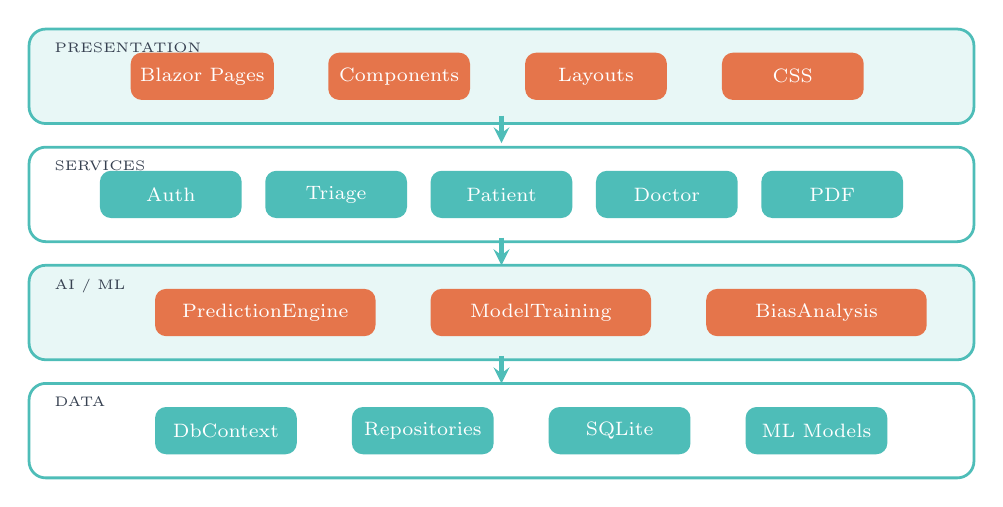
\begin{tikzpicture}[
            box/.style={rectangle, rounded corners=4pt, minimum width=1.8cm, minimum height=0.6cm, text centered, font=\scriptsize},
            layer/.style={rectangle, rounded corners=6pt, minimum width=12cm, minimum height=1.2cm, draw=primary, line width=1pt},
            arrow/.style={->, >=stealth, line width=1.5pt, primary}
        ]
        
        % Presentation Layer
        \node[layer, fill=primarybg] (pres) at (0,2.4) {};
        \node[anchor=north west, font=\tiny, darktext] at (-5.8,2.95) {PRESENTATION};
        \node[box, fill=accent, text=white] at (-3.8,2.4) {Blazor Pages};
        \node[box, fill=accent, text=white] at (-1.3,2.4) {Components};
        \node[box, fill=accent, text=white] at (1.2,2.4) {Layouts};
        \node[box, fill=accent, text=white] at (3.7,2.4) {CSS};
        
        % Service Layer
        \node[layer, fill=white] (serv) at (0,0.9) {};
        \node[anchor=north west, font=\tiny, darktext] at (-5.8,1.45) {SERVICES};
        \node[box, fill=primary, text=white] at (-4.2,0.9) {Auth};
        \node[box, fill=primary, text=white] at (-2.1,0.9) {Triage};
        \node[box, fill=primary, text=white] at (0,0.9) {Patient};
        \node[box, fill=primary, text=white] at (2.1,0.9) {Doctor};
        \node[box, fill=primary, text=white] at (4.2,0.9) {PDF};
        
        % AI Layer
        \node[layer, fill=primarybg] (ai) at (0,-0.6) {};
        \node[anchor=north west, font=\tiny, darktext] at (-5.8,-0.05) {AI / ML};
        \node[box, fill=accent, text=white, minimum width=2.8cm] at (-3,-0.6) {PredictionEngine};
        \node[box, fill=accent, text=white, minimum width=2.8cm] at (0.5,-0.6) {ModelTraining};
        \node[box, fill=accent, text=white, minimum width=2.8cm] at (4,-0.6) {BiasAnalysis};
        
        % Data Layer
        \node[layer, fill=white] (data) at (0,-2.1) {};
        \node[anchor=north west, font=\tiny, darktext] at (-5.8,-1.55) {DATA};
        \node[box, fill=primary, text=white] at (-3.5,-2.1) {DbContext};
        \node[box, fill=primary, text=white] at (-1,-2.1) {Repositories};
        \node[box, fill=primary, text=white] at (1.5,-2.1) {SQLite};
        \node[box, fill=primary, text=white] at (4,-2.1) {ML Models};
        
        % Arrows
        \draw[arrow] (0,1.9) -- (0,1.55);
        \draw[arrow] (0,0.35) -- (0,0);
        \draw[arrow] (0,-1.15) -- (0,-1.5);
        
        \end{tikzpicture}
    \end{center}
\end{frame}

%-------------------------------------------------------------------------------
% SLIDE 6: Technology Stack
%-------------------------------------------------------------------------------
\begin{frame}{Technology Stack}
    \vspace{0.3cm}
    \begin{columns}[T]
        \begin{column}{0.52\textwidth}
            {\scriptsize
            \renewcommand{\arraystretch}{1.25}
            \begin{tabular}{>{\columncolor{lightbg}}p{2.2cm} p{4.2cm}}
                \toprule
                \rowcolor{primary}
                \textcolor{white}{\textbf{Layer}} & \textcolor{white}{\textbf{Technology}} \\
                \midrule
                Framework & .NET 10.0 MAUI Blazor \\
                UI & Blazor + Scoped CSS \\
                Database & SQLite + EF Core \\
                AI/ML & ML.NET (SDCA MaxEnt) \\
                PDF & iTextSharp \\
                Auth & Custom + BCrypt \\
                \bottomrule
            \end{tabular}
            }
            
            \vspace{0.5cm}
            \begin{cleanbox}
                {\scriptsize\textbf{Why These Choices?}}
                \vspace{0.15cm}
                
                {\tiny
                \begin{itemize}
                    \setlength{\itemsep}{0.1em}
                    \item \textbf{Local-first} — No cloud dependency
                    \item \textbf{Cross-platform} — Single codebase
                    \item \textbf{Privacy} — Data stays on device
                \end{itemize}
                }
            \end{cleanbox}
        \end{column}
        \begin{column}{0.44\textwidth}
            {\scriptsize\textbf{Supported Platforms}}
            \vspace{0.3cm}
            
            {\scriptsize
            \renewcommand{\arraystretch}{1.2}
            \begin{tabular}{p{2.2cm} p{2.2cm}}
                \toprule
                \rowcolor{primary}
                \textcolor{white}{\textbf{Platform}} & \textcolor{white}{\textbf{Version}} \\
                \midrule
                \faWindows\ Windows & 10.0.17763 \\
                \faAndroid\ Android & API 24 \\
                \faApple\ iOS & 15.0 \\
                \faApple\ macOS & 15.0 \\
                \bottomrule
            \end{tabular}
            }
        \end{column}
    \end{columns}
\end{frame}

%-------------------------------------------------------------------------------
% SLIDE 7: ML Model
%-------------------------------------------------------------------------------
\begin{frame}{AI/ML Model}
    \vspace{0.2cm}
    \begin{center}
        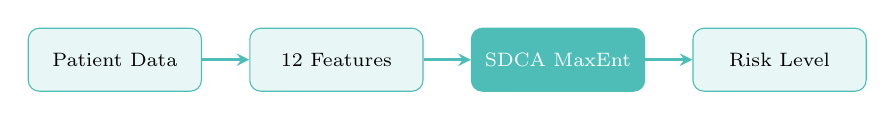
\begin{tikzpicture}[
            node distance=0.6cm,
            box/.style={rectangle, rounded corners=4pt, minimum width=2.2cm, minimum height=0.8cm, text centered, font=\scriptsize, draw=primary, fill=primarybg},
            arrow/.style={->, >=stealth, line width=1pt, primary}
        ]
        
        \node[box] (input) {Patient Data};
        \node[box, right=of input] (feat) {12 Features};
        \node[box, right=of feat, fill=primary, text=white, draw=primary] (model) {SDCA MaxEnt};
        \node[box, right=of model] (output) {Risk Level};
        
        \draw[arrow] (input) -- (feat);
        \draw[arrow] (feat) -- (model);
        \draw[arrow] (model) -- (output);
        
        \end{tikzpicture}
    \end{center}
    
    \vspace{0.3cm}
    \begin{columns}[T]
        \begin{column}{0.48\textwidth}
            {\scriptsize\textbf{Input Features (12)}}
            \vspace{0.15cm}
            
            {\tiny
            \renewcommand{\arraystretch}{1.1}
            \begin{tabular}{ll}
                \toprule
                \rowcolor{primary}
                \textcolor{white}{\textbf{Feature}} & \textcolor{white}{\textbf{Source}} \\
                \midrule
                Age, Gender & Demographics \\
                Heart Rate, BP & Vital Signs \\
                Temperature, O2 & Vital Signs \\
                Symptom Count & Assessment \\
                Symptom Severity & Weighted Score \\
                Pre-existing Count & History \\
                Diabetes, Heart, HTN & Conditions \\
                \bottomrule
            \end{tabular}
            }
        \end{column}
        \begin{column}{0.48\textwidth}
            {\scriptsize\textbf{Output Classes}}
            \vspace{0.15cm}
            
            {\tiny
            \renewcommand{\arraystretch}{1.1}
            \begin{tabular}{p{2cm} p{2.5cm}}
                \toprule
                \rowcolor{primary}
                \textcolor{white}{\textbf{Level}} & \textcolor{white}{\textbf{Response Time}} \\
                \midrule
                Emergency & Immediate \\
                Urgent & Within 15 min \\
                Standard & 30-60 min \\
                Non-Urgent & 1-2 hours \\
                \bottomrule
            \end{tabular}
            }
            
            \vspace{0.4cm}
            \begin{cleanbox}
                {\tiny\textbf{Dual System:} ML prediction + Rule-based fallback ensures reliability even without training}
            \end{cleanbox}
        \end{column}
    \end{columns}
\end{frame}

%-------------------------------------------------------------------------------
% SLIDE 8: Training Pipeline
%-------------------------------------------------------------------------------
\begin{frame}{Model Training Pipeline}
    \vspace{0.3cm}
    \begin{center}
        \begin{tikzpicture}[
            node distance=0.15cm,
            step/.style={rectangle, rounded corners=4pt, minimum width=1.5cm, minimum height=0.7cm, text centered, font=\tiny, fill=primary, text=white},
            arrow/.style={->, >=stealth, line width=0.8pt, primarydark}
        ]
        
        \node[step] (s1) {Load CSV};
        \node[step, right=of s1] (s2) {Detect\\Format};
        \node[step, right=of s2] (s3) {Transform};
        \node[step, right=of s3] (s4) {Normalize};
        \node[step, right=of s4] (s5) {Train\\80/20};
        \node[step, right=of s5] (s6) {Evaluate};
        \node[step, right=of s6] (s7) {Save};
        
        \draw[arrow] (s1) -- (s2);
        \draw[arrow] (s2) -- (s3);
        \draw[arrow] (s3) -- (s4);
        \draw[arrow] (s4) -- (s5);
        \draw[arrow] (s5) -- (s6);
        \draw[arrow] (s6) -- (s7);
        
        \end{tikzpicture}
    \end{center}
    
    \vspace{0.4cm}
    \begin{columns}[T]
        \begin{column}{0.52\textwidth}
            {\scriptsize\textbf{CSV Training Data Format}}
            \vspace{0.15cm}
            
            {\tiny
            \renewcommand{\arraystretch}{1.1}
            \begin{tabular}{p{2cm} p{4cm}}
                \toprule
                \rowcolor{primary}
                \textcolor{white}{\textbf{Column}} & \textcolor{white}{\textbf{Description}} \\
                \midrule
                Patient\_ID & Unique identifier \\
                Age & Patient age in years \\
                Gender & Male / Female \\
                Symptoms & Comma-separated list \\
                Blood\_Pressure & Format: "120/80" \\
                Heart\_Rate & Beats per minute \\
                Temperature & Celsius \\
                Pre\_Existing & Conditions list \\
                Risk\_Level & Low/Medium/High/Critical \\
                \bottomrule
            \end{tabular}
            }
        \end{column}
        \begin{column}{0.44\textwidth}
            \begin{cleanbox}
                {\scriptsize\textbf{Smart Features}}
                \vspace{0.2cm}
                
                {\tiny
                \begin{itemize}
                    \setlength{\itemsep}{0.15em}
                    \item \textbf{Auto-separator} — CSV or TSV
                    \item \textbf{Symptom weighting} — Severe: +3, Moderate: +2
                    \item \textbf{Reproducible} — Seed = 42
                    \item \textbf{Min-Max normalization} — Features scaled 0-1
                \end{itemize}
                }
            \end{cleanbox}
        \end{column}
    \end{columns}
\end{frame}

%-------------------------------------------------------------------------------
% SLIDE 9: Bias Analysis
%-------------------------------------------------------------------------------
\begin{frame}{Bias \& Fairness Analysis}
    \vspace{0.2cm}
    \begin{center}
        \begin{cleanbox}[colback=white]
            \centering
            {\small\textbf{Proactive AI Ethics:} Built-in demographic fairness monitoring}
        \end{cleanbox}
    \end{center}
    
    \vspace{0.3cm}
    \begin{columns}[T]
        \begin{column}{0.48\textwidth}
            {\scriptsize\textbf{Metrics Analyzed}}
            \vspace{0.15cm}
            
            {\tiny
            \renewcommand{\arraystretch}{1.15}
            \begin{tabular}{p{2cm} p{3.2cm}}
                \toprule
                \rowcolor{primary}
                \textcolor{white}{\textbf{Dimension}} & \textcolor{white}{\textbf{Groups}} \\
                \midrule
                Gender & Male vs Female \\
                Age Groups & 0-17, 18-34, 35-49, 50-64, 65+ \\
                \bottomrule
            \end{tabular}
            }
            
            \vspace{0.3cm}
            {\scriptsize\textbf{Per-Group Metrics}}
            {\tiny
            \begin{itemize}
                \setlength{\itemsep}{0.1em}
                \item Prediction Accuracy (\%)
                \item False Positive Rate
                \item False Negative Rate
                \item Risk Distribution
            \end{itemize}
            }
        \end{column}
        \begin{column}{0.48\textwidth}
            {\scriptsize\textbf{Fairness Score}}
            \vspace{0.15cm}
            
            \begin{cleanbox}
                {\tiny
                Score = 100\\
                \hspace{0.3cm}$-$ (Gender Gap $\times$ 2)\\
                \hspace{0.3cm}$-$ FP Disparity\\
                \hspace{0.3cm}$-$ FN Disparity\\
                \hspace{0.3cm}$-$ (Age Variance $\times$ 0.5)
                }
            \end{cleanbox}
            
            \vspace{0.2cm}
            {\tiny
            \renewcommand{\arraystretch}{1.1}
            \begin{tabular}{p{1.5cm} p{2.5cm}}
                \toprule
                \rowcolor{primary}
                \textcolor{white}{\textbf{Score}} & \textcolor{white}{\textbf{Rating}} \\
                \midrule
                $\geq$90 & Excellent \\
                80-89 & Good \\
                70-79 & Fair \\
                60-69 & Needs Improvement \\
                $<$60 & Poor \\
                \bottomrule
            \end{tabular}
            }
        \end{column}
    \end{columns}
\end{frame}

%-------------------------------------------------------------------------------
% SLIDE 10: Department Routing
%-------------------------------------------------------------------------------
\begin{frame}{Smart Department Routing}
    \vspace{0.2cm}
    \begin{columns}[T]
        \begin{column}{0.55\textwidth}
            {\scriptsize\textbf{Weighted Scoring Algorithm}}
            \vspace{0.15cm}
            
            {\tiny
            \renewcommand{\arraystretch}{1.1}
            \begin{tabular}{p{2cm} p{4.2cm}}
                \toprule
                \rowcolor{primary}
                \textcolor{white}{\textbf{Department}} & \textcolor{white}{\textbf{Key Triggers}} \\
                \midrule
                Emergency & O2 $<$90\%, severe bleeding, unconscious \\
                Cardiology & Chest pain, HR $>$110/$<$55, BP $>$160 \\
                Pulmonology & Shortness of breath, O2 90-94\% \\
                Neurology & Altered consciousness, stroke signs \\
                Orthopedics & Severe isolated pain \\
                General Med & Fever, mild abnormal vitals \\
                \bottomrule
            \end{tabular}
            }
            
            \vspace{0.3cm}
            {\tiny\textbf{Priority:} Emergency $\rightarrow$ Cardiology $\rightarrow$ Pulmonology $\rightarrow$ Neurology $\rightarrow$ Orthopedics $\rightarrow$ General}
        \end{column}
        \begin{column}{0.42\textwidth}
            \begin{cleanbox}
                {\scriptsize\textbf{Explainable Recommendations}}
                \vspace{0.2cm}
                
                {\tiny
                Every routing decision includes:
                \begin{itemize}
                    \setlength{\itemsep}{0.1em}
                    \item Human-readable explanation
                    \item Actual patient values cited
                    \item Confidence percentage
                    \item All department scores (audit)
                \end{itemize}
                }
            \end{cleanbox}
            
            \vspace{0.3cm}
            \centering
            {\scriptsize\textbf{6 Supported Departments}\\+ ICU for critical cases}
        \end{column}
    \end{columns}
\end{frame}

%-------------------------------------------------------------------------------
% SLIDE 11: User Workflow
%-------------------------------------------------------------------------------
\begin{frame}{User Workflow}
    \vspace{0.3cm}
    \begin{center}
        \begin{tikzpicture}[
            node distance=0.8cm,
            step/.style={rectangle, rounded corners=3pt, minimum width=1.8cm, minimum height=1cm, text centered, font=\tiny, draw=border, fill=lightbg},
            arrow/.style={->, >=stealth, line width=1pt, primary}
        ]
        
        \node[step] (s1) {\textcolor{primary}{\faUserPlus}\\[0.1em]\textbf{Intake}};
        \node[step, right=of s1] (s2) {\textcolor{primary}{\faStethoscope}\\[0.1em]\textbf{Assessment}};
        \node[step, right=of s2, fill=primary, text=white, draw=primary] (s3) {\textcolor{white}{\faBrain}\\[0.1em]\textbf{AI Triage}};
        \node[step, right=of s3, fill=accent, text=white, draw=accent] (s4) {\textcolor{white}{\faHospital}\\[0.1em]\textbf{Routing}};
        \node[step, right=of s4] (s5) {\textcolor{primary}{\faUserMd}\\[0.1em]\textbf{Assign}};
        
        \draw[arrow] (s1) -- (s2);
        \draw[arrow] (s2) -- (s3);
        \draw[arrow] (s3) -- (s4);
        \draw[arrow] (s4) -- (s5);
        
        \end{tikzpicture}
    \end{center}
    
    \vspace{0.5cm}
    \begin{columns}[T]
        \begin{column}{0.32\textwidth}
            \centering
            {\small\textcolor{primary}{\faUser}}\\[0.2em]
            {\scriptsize\textbf{Patient Role}}
            
            {\tiny
            \begin{itemize}
                \setlength{\itemsep}{0.1em}
                \item Self-service portal
                \item View triage status
                \item See assigned doctor
                \item Download reports
            \end{itemize}
            }
        \end{column}
        \begin{column}{0.32\textwidth}
            \centering
            {\small\textcolor{primary}{\faUserMd}}\\[0.2em]
            {\scriptsize\textbf{Doctor Role}}
            
            {\tiny
            \begin{itemize}
                \setlength{\itemsep}{0.1em}
                \item View assigned patients
                \item Access medical history
                \item Review assessments
                \item Update status
            \end{itemize}
            }
        \end{column}
        \begin{column}{0.32\textwidth}
            \centering
            {\small\textcolor{primary}{\faUserCog}}\\[0.2em]
            {\scriptsize\textbf{Admin Role}}
            
            {\tiny
            \begin{itemize}
                \setlength{\itemsep}{0.1em}
                \item Full dashboard access
                \item Manage doctors
                \item Train AI models
                \item Analyze bias metrics
            \end{itemize}
            }
        \end{column}
    \end{columns}
\end{frame}

%-------------------------------------------------------------------------------
% SLIDE 12: Screenshots
%-------------------------------------------------------------------------------
\begin{frame}{Application Screenshots}
    \vspace{0.3cm}
    \begin{center}
        {\small\textcolor{primary}{[ADD SCREENSHOTS HERE]}}
        
        \vspace{0.6cm}
        \begin{columns}[T]
            \begin{column}{0.32\textwidth}
                
\begin{tikzpicture}
                    \node[rectangle, rounded corners=6pt, minimum width=3.5cm, minimum height=2cm, draw=primary, line width=1pt, fill=primarybg] {
                        {\tiny\textcolor{primarydark}{Home Page}}
                    };
                \end{tikzpicture}
            \end{column}
            \begin{column}{0.32\textwidth}
                
\begin{tikzpicture}
                    \node[rectangle, rounded corners=6pt, minimum width=3.5cm, minimum height=2cm, draw=primary, line width=1pt, fill=primarybg] {
                        {\tiny\textcolor{primarydark}{Triage Assessment}}
                    };
                \end{tikzpicture}
            \end{column}
            \begin{column}{0.32\textwidth}
                
\begin{tikzpicture}
                    \node[rectangle, rounded corners=6pt, minimum width=3.5cm, minimum height=2cm, draw=primary, line width=1pt, fill=primarybg] {
                        {\tiny\textcolor{primarydark}{AI Model Page}}
                    };
                \end{tikzpicture}
            \end{column}
        \end{columns}
        
        \vspace{0.5cm}
        \begin{columns}[T]
            \begin{column}{0.32\textwidth}
                
\begin{tikzpicture}
                    \node[rectangle, rounded corners=6pt, minimum width=3.5cm, minimum height=2cm, draw=primary, line width=1pt, fill=primarybg] {
                        {\tiny\textcolor{primarydark}{Admin Dashboard}}
                    };
                \end{tikzpicture}
            \end{column}
            \begin{column}{0.32\textwidth}
                
\begin{tikzpicture}
                    \node[rectangle, rounded corners=6pt, minimum width=3.5cm, minimum height=2cm, draw=primary, line width=1pt, fill=primarybg] {
                        {\tiny\textcolor{primarydark}{Doctor Management}}
                    };
                \end{tikzpicture}
            \end{column}
            \begin{column}{0.32\textwidth}
                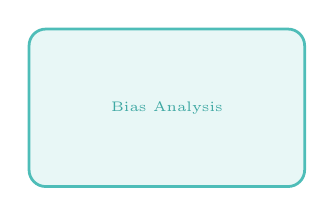
\begin{tikzpicture}
                    \node[rectangle, rounded corners=6pt, minimum width=3.5cm, minimum height=2cm, draw=primary, line width=1pt, fill=primarybg] {
                        {\tiny\textcolor{primarydark}{Bias Analysis}}
                    };
                \end{tikzpicture}
            \end{column}
        \end{columns}
    \end{center}
\end{frame}

%-------------------------------------------------------------------------------
% SLIDE 13: Unique Innovations
%-------------------------------------------------------------------------------
\begin{frame}{What Makes CareSync Unique}
    \vspace{0.2cm}
    \begin{columns}[T]
        \begin{column}{0.48\textwidth}
            \begin{cleanbox}
                {\scriptsize\textcolor{accent}{\faShieldAlt}\ \textbf{Dual Prediction System}}
                \vspace{0.15cm}
                
                {\tiny ML model + clinical rules fallback ensures it \textbf{always works} — even without training data}
            \end{cleanbox}
            
            \vspace{0.2cm}
            \begin{cleanbox}
                {\scriptsize\textcolor{accent}{\faBalanceScale}\ \textbf{Built-in Bias Monitoring}}
                \vspace{0.15cm}
                
                {\tiny Automatic demographic fairness analysis — rare in healthcare AI, shows proactive ethics}
            \end{cleanbox}
            
            \vspace{0.2cm}
            \begin{cleanbox}
                {\scriptsize\textcolor{accent}{\faComments}\ \textbf{Explainable AI}}
                \vspace{0.15cm}
                
                {\tiny Every prediction includes \textbf{human-readable explanations} with actual patient values}
            \end{cleanbox}
        \end{column}
        \begin{column}{0.48\textwidth}
            \begin{cleanbox}
                {\scriptsize\textcolor{accent}{\faMicrochip}\ \textbf{On-Device AI}}
                \vspace{0.15cm}
                
                {\tiny ML.NET runs \textbf{locally} — no cloud dependency, works offline, data stays private}
            \end{cleanbox}
            
            \vspace{0.2cm}
            \begin{cleanbox}
                {\scriptsize\textcolor{accent}{\faFileAlt}\ \textbf{Full Audit Trail}}
                \vspace{0.15cm}
                
                {\tiny JSON-serialized scores for every decision — full transparency for compliance}
            \end{cleanbox}
            
            \vspace{0.2cm}
            \begin{cleanbox}
                {\scriptsize\textcolor{accent}{\faHistory}\ \textbf{Model Versioning}}
                \vspace{0.15cm}
                
                {\tiny Tracks training date, record count, accuracy metrics for regulatory compliance}
            \end{cleanbox}
        \end{column}
    \end{columns}
\end{frame}

%-------------------------------------------------------------------------------
% SLIDE 14: Future Scope
%-------------------------------------------------------------------------------
\begin{frame}{Future Roadmap}
    \vspace{0.2cm}
    \begin{columns}[T]
        \begin{column}{0.48\textwidth}
            {\scriptsize\textbf{Phase 1: Enhanced AI}}
            {\tiny
            \begin{itemize}
                \setlength{\itemsep}{0.1em}
                \item Deep learning (TensorFlow.NET)
                \item NLP symptom processing
                \item Image-based diagnosis
                \item Voice input
            \end{itemize}
            }
            
            \vspace{0.3cm}
            {\scriptsize\textbf{Phase 2: Integration}}
            {\tiny
            \begin{itemize}
                \setlength{\itemsep}{0.1em}
                \item HL7 FHIR compliance
                \item Hospital EHR/EMR sync
                \item Bed availability API
                \item Insurance verification
            \end{itemize}
            }
        \end{column}
        \begin{column}{0.48\textwidth}
            {\scriptsize\textbf{Phase 3: Analytics}}
            {\tiny
            \begin{itemize}
                \setlength{\itemsep}{0.1em}
                \item Wait time prediction
                \item Resource forecasting
                \item Outbreak detection
                \item Performance benchmarks
            \end{itemize}
            }
            
            \vspace{0.3cm}
            {\scriptsize\textbf{Phase 4: Scale}}
            {\tiny
            \begin{itemize}
                \setlength{\itemsep}{0.1em}
                \item Multi-hospital deployment
                \item Azure cloud sync option
                \item Federated learning
                \item Telemedicine integration
            \end{itemize}
            }
        \end{column}
    \end{columns}
    
    \vspace{0.5cm}
    \begin{center}
        \begin{cleanbox}[colback=white]
            \centering
            {\scriptsize\textcolor{accent}{\faRocket}\ \textbf{Vision:} From hackathon prototype to production-ready hospital solution}
        \end{cleanbox}
    \end{center}
\end{frame}

%-------------------------------------------------------------------------------
% SLIDE 15: Thank You
%-------------------------------------------------------------------------------
{
\setbeamercolor{background canvas}{bg=primary}
\begin{frame}[plain]
    \vspace{2.5cm}
    \begin{center}
        {\fontsize{32}{38}\selectfont\textcolor{white}{\textbf{Thank You}}}
        
        \vspace{1.2cm}
        \textcolor{accent}{\rule{3cm}{3pt}}
        
        \vspace{1cm}
        {\normalsize\textcolor{white}{Team \textbf{KludgeKings}}}
        
        \vspace{1.5cm}
        {\small\textcolor{primarybg}{Questions?}}
        
        \vspace{1cm}
        {\scriptsize\textcolor{primarylight}{CareSync — AI-Powered Smart Patient Triage System}}
    \end{center}
\end{frame}
}

\end{document}
